
%%%%%%%%%%%%%%%%%%%%%%%%%%%%%%%%%%%%%%%%%%
\section{Results}
\label{sec:cub:results}
%%%%%%%%%%%%%%%%%%%%%%%%%%%%%%%%%%%%%%%%%%

\begin{figure}[t]
    \centering
    \subfloat[Test cases commonality scores.]{
        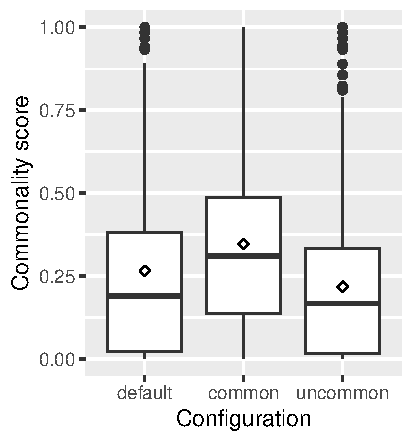
\includegraphics[height=50mm]{papers/cub/images/score.pdf}
        \label{subfig:score}
    }
    \subfloat[Effect sizes $\widehat{A}_{12}$ .]{
        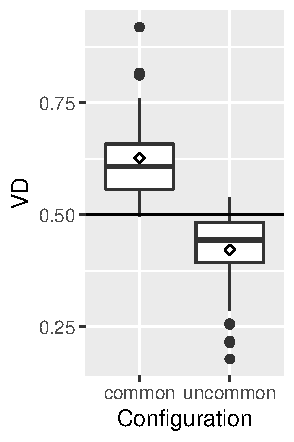
\includegraphics[height=50mm]{papers/cub/images/score-vd.pdf}
        \label{subfig:scorevd}
    }\\
    \subfloat[Effect sizes $\widehat{A}_{12}$ magnitudes.% (\textit{Significant differences $<0.05$}.
    ]{
        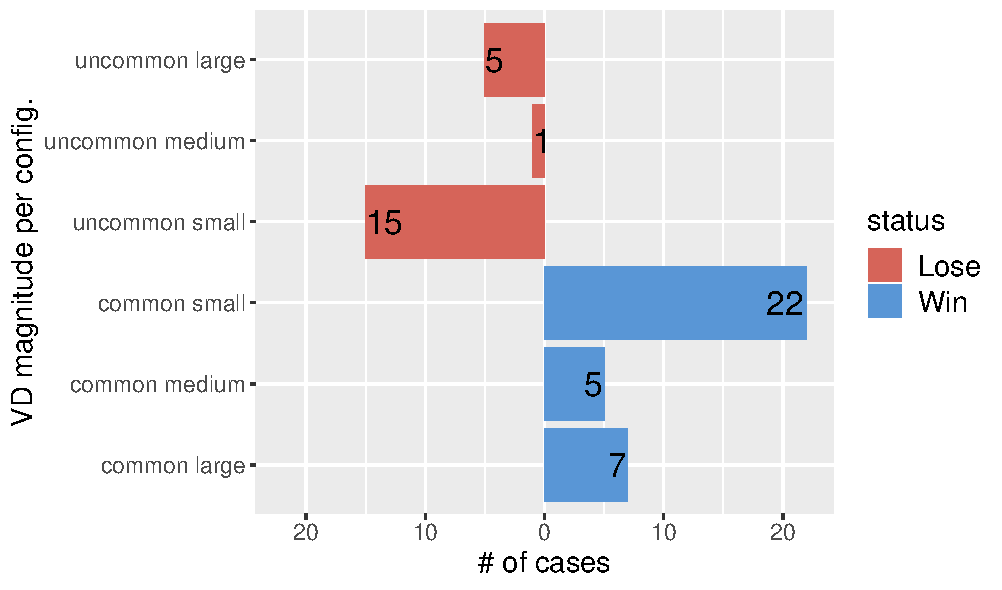
\includegraphics[height=50mm]{papers/cub/images/score-sig.pdf}
        \label{subfig:scoresig}
    } 
    
    \caption{Test cases commonality values and comparison to \df. Diamonds indicate mean values and horizontal bars (\textbf{--}) indicate median values.}
    \label{fig:rq1}
\end{figure}

\subsection{Commonality Score (RQ1)}

In this section we answer the question: \emph{How does the \emph{commonality score} of the generated tests compare when using the \textit{common}, \textit{uncommon}, and \textit{default} secondary objectives?}

Figure \ref{fig:rq1} illustrates the impact of using \com and \ucom, as the secondary objective, on the commonality score of the generated test cases. Figure \ref{subfig:score} shows that the average and median of the commonality score is improved by 8\% and 12\%, respectively, compared to \df when using \com as secondary objective.
In parallel, using \ucom as secondary objective reduces the commonality score by, on average, 5\% (2.5\% for median) compared to \df. Moreover, Figure \ref{subfig:scoresig} presents the number of cases (\ie classes used as the target class for unit testing), in which the application of \com and \ucom significantly (\textit{p-value} $<0.05$) changes the commonality score with effect size magnitude of large, medium, or small. As we can see in this figure, utilizing \com always leads to a significant improvement in the commonality score (blue bars), and in contrast, using \ucom always reduces this score (red bars). In total, \com significantly improves the commonality score in 34 cases (32.6\% of classes), and \ucom significantly reduces this score in 21 classes (20.1\% of cases). Figure \ref{subfig:scorevd} depicts the effect sizes of differences observed in these cases. Consistent with the previous figures, the average effect size ($\widehat{A}_{12}$) achieved by \com is higher than 0.5 (\ie commonality score has been improved). However, this value is lower than 0.5 for \ucom.

\paragraph{Summary} Using \com as secondary objective in the \evosuite search-based test case generation process leads to test cases that exhibit an improved commonality score. In parallel, the application of \ucom leads to the reduction of the commonality score.

%-----------------------------------------
\subsection{Structural Coverage (RQ2)}
%-----------------------------------------

In this section we provide an answer to the following research question: \emph{How does the \emph{line} and \emph{branch coverage} of the generated tests  compare when using the \textit{common}, \textit{uncommon}, and \textit{default} secondary objectives?}

Figure~\ref{fig:rq2} shows the line and branch coverage achieved by using \com and \ucom as secondary objectives compared to \df. Figure~\ref{subfig:coverage} indicates that the average coverage is the same for all of the assessed configurations.

Looking at the comparison of the structural coverage values achieved by each secondary objective in each class, we can see that the line and branch coverage is significantly impacted by \com and \ucom in some cases. Figure~\ref{subfig:coveragesig} presents the number of cases that these secondary objectives significantly (\textit{p-value} $<0.05$) reduce ($\widehat{A}_{12} < 0.5$) or increase ($\widehat{A}_{12} > 0.5$) the line and branch coverage with effect size magnitude small, medium, or large. According to this figure, in general, utilizing \com leads to a significant improvement for line and branch coverage in three and four classes, respectively. Nevertheless, this secondary objective reduced the line and branch coverage in eight and nine classes, respectively. 

Also, we can see a similar result for \ucom:
significant improvements in three and five classes and significant reductions in seven and nine cases for line and branch coverage. Since the number of cases in which \com and \ucom lead to a significantly lower structural coverage is higher than the the number of cases in which we see a significant improvement in coverage, the average effect size of differences (Figure~\ref{subfig:coveragevd}) is slightly less than  $0.5$ for both line (0.47 for both secondary objectives) and branch coverage (0.46 for both).

\paragraph{Summary} On average, using \com or \ucom does not impact the line and branch coverage. However, these two secondary objectives can significantly impact the structural coverage in specific cases.

\begin{figure}[t]
    \centering
    \subfloat[Test suites coverage and mutation score.]{
        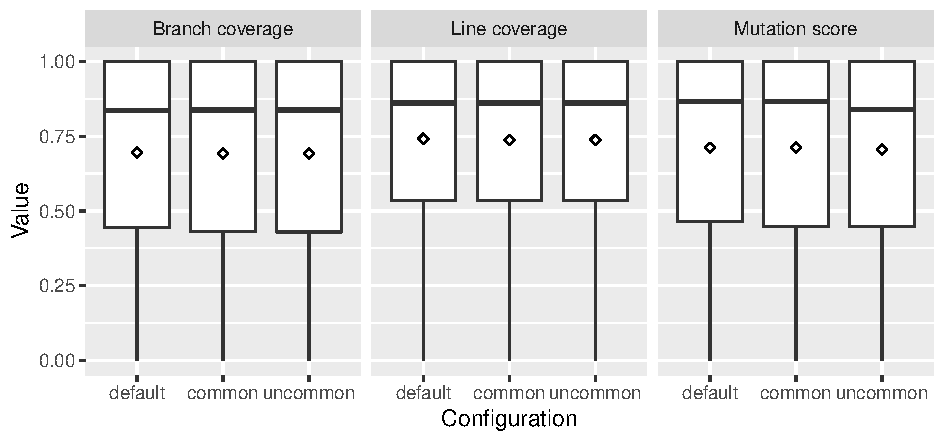
\includegraphics[height=30mm]{papers/cub/images/coverage.pdf}
        \label{subfig:coverage}
    }\hfill
    \subfloat[Effect sizes $\widehat{A}_{12}$.]{
        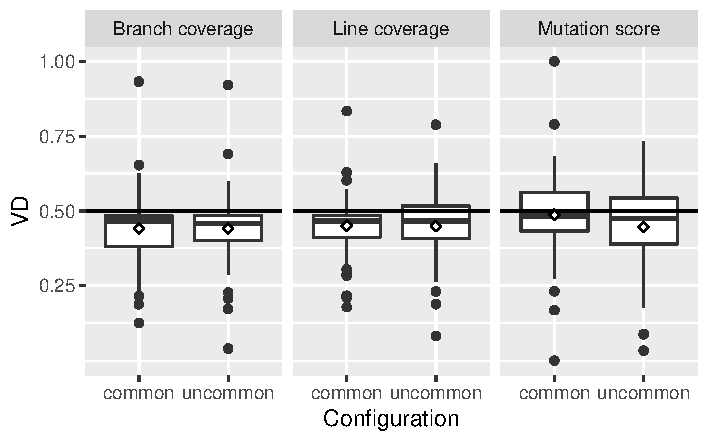
\includegraphics[height=30mm]{papers/cub/images/coverage-vd.pdf}
        \label{subfig:coveragevd}
    }\\ 
    \subfloat[Effect sizes $\widehat{A}_{12}$ magnitudes.]{
        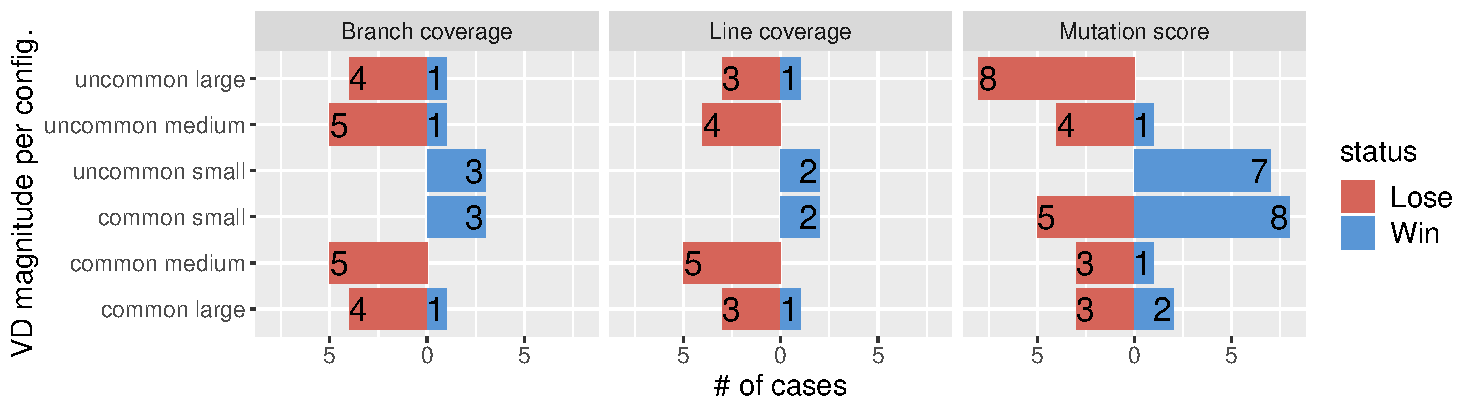
\includegraphics[height=30mm]{papers/cub/images/coverage-sig.pdf}
        \label{subfig:coveragesig}
    }
   
    \caption{Test suites coverage and mutation score, and comparison to \textit{default}. Diamonds indicate mean values and horizontal bars (\textbf{--}) indicate median values.}
    \label{fig:rq2}
\end{figure}

%-----------------------------------------
\subsection{Mutation Analysis (RQ3)}
%-----------------------------------------

In the final research question we reflect on \emph{How does the \emph{mutation score} of the generated tests  compare when using the \textit{common}, \textit{uncommon}, and \textit{default} secondary objectives? }

Figure \ref{subfig:coverage} depicts the mutation score achieved by using \com and \ucom compared to \df. Like line and branch coverage, the average mutation scores achieved by these secondary objectives is similar to the one achieved by \df. 
However, Figure \ref{subfig:coveragesig} shows that \com and \ucom can significantly (\textit{p-value} $<0.05$) impact the mutation score achieved by unit test generation. The \com secondary objective significantly increases the number of mutants killed for 11 classes but, at the same time, also decreases the mutation score in another 11 cases. Moreover, \ucom significantly changes the mutation score in 20 cases (8 wins against 12 losses). 
Figure \ref{subfig:coveragevd} shows the effect size of differences in these cases for both \com and \ucom secondary objectives. According to this Figure, the average $\widehat{A}_{12}$ estimations are 0.49 and 0.47. Since these values are lower than 0.5, on average, the difference achieved by these two secondary objectives is negative. However, the outliers in this figure show us that the effect sizes of \com above 0.75 in some specific cases. Hence, the graphs in Figure~\ref{subfig:coveragesig} indicate that using \com and \ucom can improve the mutation score in specific cases.

\paragraph{Summary} On average, using \com or \ucom does not have any effect on the mutation score achieved by the generated test suites. However, these two secondary objectives can significantly change the killed mutants in some cases.